\chapter{Inertial Waves in a Rotating Cone}

\section{Introduction}

Following the introduction and validation of the immersed boundary methods,
we now want to exemplary investigate a rotating fluid system using these methods.
The objective is to reproduce  physical properties, with respect to theoretical and experimental results.
In relation to the research focus of the geophysical fluid mechanics research group, there are a variety
topics of interest.\\
One area of research lies in the exploration of dynamo effects in geological and stellar system.
In particular this means the generation of magnetic fields by electrically conducting fluids on large scales.
In this thesis we will not consider MHD-equations.  \footnote{MHD - Magnetohydrodynamics}
However in general it is considered that the helicity of a fluid domain $\Omega$, given by

\begin{align}
    \int_{\Omega}\dif V  \vec{u} \left( \nabla \times \vec{u} \right)
\end{align}

is directly linked to dynamo action \citep{moffat1978}.
It would be interesting to find a system which exhibits a large helicity,
as a possible candidate for future researches of the geodynamo.
Furthermore we are interested in the propagation of inertial waves in different fluid domains.\\
The systems we want to study in this thesis is given by a rotating cone, which is compared to
a frustum, by inserting a bottom plate into the apex.
Inertial waves are excited by a temporal modulation of the rotation frequency, which is denoted as libration.
The objective is to examine the ability to generate inertial modes or wave attractors.
Furthermore we want to study the properties of the helicity of the system and investigate the
decay of inertial oscillations.\\
In this chapter we will use linearized equations. Due to the axial symmetry with the rotating axis,
this problem could be reduced to two dimensions.
However, we want to test the code in a three dimensional setup.
One reason for this is a possible future application.
Th objective would be to study the decay of turbulence in the apex of the cone.
A simulation in three dimensions can not be avoided in this case.

\section{Theoretical Description}
\label{cone:theorie_theo}

This section gives a brief theoretical description of the problem adapted from \citep{Greenspan1969}, \citep{Beardsley1970}.
Instead of a cone, a comparison to the two-dimensional analogy of a wedge, is made.
This system is based on the idea to introduce a geometric shape, which contains a singularity.\\
Let us consider the propagation of an inertial wave ray, emitted at one of the upper edges of
the wedge, as shown in figure \ref{cone:theorie}.
The wave propagates under the angle $\theta = \arccos(\omega/2)$, with respect to the horizontal axis.
For each reflection the propagation angle with respect to the rotation axis is preserved.
In the case of $\theta<\alpha$ we have a supercritical reflection,
thus a downward traveling wave ray is reflected downslope.

\begin{figure}[!bp]
  \begin{minipage}[c]{0.6\textwidth}
      \centering
        \resizebox{0.7\textwidth}{!}{
       \import{gfx/cone//}{cone.pdf_tex}
      }
  \end{minipage}
  \begin{minipage}[c]{0.3\textwidth}
      \caption{
          Propagation of an inertial wave emitted from the top edge of a wedge,
           where $\Theta$ indicates the direction parallel to the group velocity
            $\vec{c_g}$.  $L$ and $L^{\prime}$ are the path lengths before and after a reflection.
      \label{cone:theorie}
      }
  \end{minipage}
\end{figure}

As a results the wave travels towards the lower vertex of the wedge.
It can be shown from the reflection properties, given by equation \ref{theorie:reflections},
that the time for a wave ray to travel the path between two reflections is constant \citep{Beardsley1970}.
To be more precisely

\begin{align}
    \frac{L}{|\vec{c}_g|} = \frac{L^{\prime}}{|\vec{c}_g^{\prime}|}
\end{align}

the prime denotes the properties after a reflection.
This means that the overall propagation time into the apex of the cone becomes infinity, along with the energy density and the wave number.
Thus, the apex is acting as an attractor to inertial waves.
As a conclusion it follows that since no reflection out of the cone apex can occur, the possibility of inertial modes is not given.

\section{Experiment}
\label{cone:theorie_exp}

For a test of these theoretical assumptions, an experimental study was performed by \citep{Beardsley1970}.
The schematic setup is shown in figure \ref{cone:setup_experiment}.
In the first part of the experiment a plexiglass cylinder, containing a conical shaped cavity,
of height $H=\SI{19.95}{\centi\meter}$ and a radius of $r=\SI{19.95}{\centi\meter}$ was used.
The apex half angle was set to $\alpha=24^{\circ}3.7^{\prime}$ degree.
For the rotation rate a frequency of $\Omega_0 =\SI{6.28}{\radian\per\second}$ was chosen.
As a fluid, water was used, the resulting viscosity, given by \citep{tipler2003}, is $\nu = \SI{1.0}{\milli\pascal\second}$.
The resulting Ekman number is

\begin{align}
    \Ekman = \frac{\nu}{\omega r H^2} \approx 7.72\cdot 10^{-6}
\end{align}

In order to exite inertial waves the cone is librating.
The total rotation rate is proportional to

\begin{align}
\Omega(t) = \Omega_0 + \epsilon_0 \omega \cos(\omega t)
\end{align}

where $\omega$ is the libration frequency with the amplitude $\epsilon_0=\SI{0.2}{\radian}$.
The excitation mechanism is a result from the wall friction, induced
by the modulation of the constant rotation frequency $\Omega_0$.

\begin{figure}[!b]
      \centering
        \resizebox{0.6\textwidth}{!}{
       \import{gfx/cone///}{experiment.pdf_tex}
      }
      \caption{
          Experimental Setup. In the first experiment a cone is used (left). For the second part the apex of the cone
          is replaced by a frustum (right).
      \label{cone:setup_experiment}
      }
\end{figure}

For the analysis the dynamic pressure field was measured at different depths along the rotation axis.
The ratio of libration to the constant rotation frequency was varied in the range of ${0.25\leq\omega/2\Omega_0\leq1}$.
The pressure and phase lag spectrum  show that no consistent peaks are observable for different measurment heights.
Hence, no inertial modes are existing.
\\
In the second part of the experiment, the apex of the cone was replaced by a frustum, through the
insertion of a bottom plate in the cone at the position $z/H = 0.261$.
This setup yields the possibility that a wave ray can be reflected on the bottom.
The pressure and phase lag spectrum in this setup show that
independent of the height resonances occur which can be associated with standing waves.
Hence, inertial modes exist.

\clearpage

\section{Numerical Implementation of Libration}

For the numerical implementation of the experiment, a modified set of the equations
introduced in section \ref{THEORIE:ROT}, is presented here.
It has to be concerned, that the system has now a time-dependent rotation rate.
For the non-dimensional system, with $\vec{u}^* =  \vec{u} (|\vec{\Omega}|L)^{-1}$, we set

\begin{align}
    \vec{\Omega(t)} = 1 \; + \; \epsilon \cos(\omega t)\vec{e}_z
\end{align}

There are two options for an implementation.
First of all, we can choose a rotating coordinate system with a constant velocity $\Omega_0$.
This means the we can directly use the equations \ref{theorie:rotns}. Since the overall rotation rate of the system is
modulated, it is necessary to introduce the boundary conditions

\begin{align}
    \vec{v}|_{Border}  = \Omega \times \vec{r} = \begin{pmatrix}
           -y \epsilon \cos(\omega t) \\
           x \epsilon \cos(\omega t) \\
           0\\
         \end{pmatrix}
\end{align}

However, obtaining a linearized version of the boundary methods is not as easy.
In addition we think it is safer to use No-Slip boundaries with zero velocity, as
the taylor-couette system showed that velocities other than zero, can create a larger numerical error.
The alternative option is the introduction of an accelerated frame of reference.
In this case the boundary conditions do not need to be modified, but the coriolis forcing term is given by \citep{Tilgner2007}.

\begin{align}
    \vec{f} &= 2 \vec{\Omega} \times \vec{v} + \pdn[]{t}\left(\vec{\Omega} \times \vec{v} \right)
            = \begin{pmatrix}
           -y \omega \epsilon \cos(\omega t) \\
           -x \omega \epsilon \cos(\omega t) \\
           0\\
         \end{pmatrix}
            + 2\begin{pmatrix}
           - ( 1 + \epsilon \sin(\omega t)v_x \\
             ( 1 + \epsilon \sin(\omega t)v_y \\
           0\\
         \end{pmatrix}
            = \begin{pmatrix}
           -y \epsilon \cos(\omega t) \\
           -x \epsilon \cos(\omega t) \\
           0\\
         \end{pmatrix}
\end{align}

In the last step the linearization was introduced.
The non-linear advection term is removed from the equations of motion, which
are then given by

\begin{align}
    \label{theorie:rotns}
    \pdn[u]{t} = -c^2\nabla \rho + \Ekman \Delta \vec{u} + \vec{f} \qquad;& \qquad  \nabla \vec{v} = 0
\end{align}

Finally one additional stability criterion shall be introduced,
It is important that the time for propagating information from on side of the domain
to the other, is much smaller than the overall rotation rate.
\footnote{Private communication with A. Tilgner}
This can be estimated by

\begin{align}
    t = \sqrt{\frac{2}{c^2}} << 2\pi
\end{align}

Thus the propagation time and therefore this criterion, depends on the artificial sound speed.
A good estimation is given by setting $c^2 = 500$.
It could be observed that otherwise, not only physical wrong results are obtained but also
numerical instabilities can occur.
\footnote{Private communication with O. Goepfert}

\newpage

\section{Setup}

This section introduces the setup which has been used for the simulations presented in this chapter.
Figure \ref{cone:setup_image} shows the geometry of the fluid domain.
In the remaining sections of this chapter we want to use the following conventions:

\begin{multicols}{2}
\begin{description}
    \item[$H$]{Total height of the simulation domain}
    \item[$h_c$]{Height of the Cone}
    \item[$h_b$]{Height of the bottom plate}
    \item[$r$]{Radius of the bottom plate}
    \item[$O$]{Offset at the top of the Cone}
    \item[$\alpha$]{Slope of the Cone}
    \item[$\Theta$]{Propagation angle of an inertial wave, with respect to the horizontal axis.}
    \item[$\Omega$]{Rotation rate}
    \item[$\omega$]{Frequency of the libration}
    \item[$\epsilon$]{Amplitude of the libration, default is 1\footnote{Not important due to the linearization}}
    \item[Cone] {The entire cone with apex, and a possible offset at the top}
    \item[Frustum]{The apex of the cone is replaced by bottom plate at height $h_t$}
\end{description}
\end{multicols}

%For the implementation the testcase function template introduced in chapter () is used.
%The use of the different parameters with this template is shown in Appendix ().

\begin{figure}[!bp]
  \centering
        \resizebox{0.6\textwidth}{!}{
       \import{gfx/cone/conesim//}{setup.pdf_tex}
      }
      \caption{Numerical Setup for the Simulations \label{cone:setup_image} }
\end{figure}
\clearpage

\section{Data Analysis}

The main interest, in the analysis of the simulation data, lies in the identification of possible inertial modes.
A appropriate choice is to consider the energy in the $z$-component of the  velocity, which is given by

\begin{align}
    \left<v_z^2 \right>(t) =  \int \dif V v_z(t)^2 \approx \sum_{i, j, k}^{N_x,N_y,N_z} \Delta x \Delta y \Delta z \left.v_z(t)^2 \right|_{i,j,k}
\end{align}

This has multiple benefits

\begin{itemize}
    \item The $v_z$-velocity component is independent of the coordinate system which is used, it is not necessary
                to compute a transformation to inertial frame.
    \item The energy induced by the libration is perpendicular to this component, thus all components
            in the $v_z$-component are created by inertial oscillations.
\end{itemize}

In figure \ref{fig:cone:cyl_vzmode}, this energy is shown exemplarly for two libration frequencies for a cylinder.
\footnote{The results are taken from section \ref{cone:sec:lib_cylinder}}
For a resonance of the system ($\omega=1.2$), it takes further time until a steady state, with a constant oscillation is reached.

\begin{figure}[!pb]
  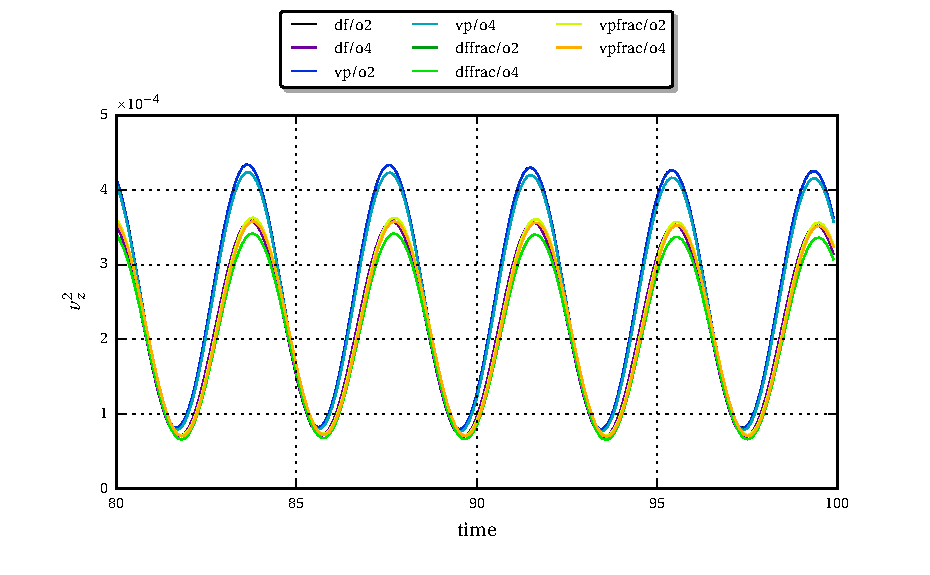
\includegraphics{gfx/cone/cylinder/cyl_vz.pdf}
  \caption{Kinetic energy in $z$-direction for the direct forcing 2nd-order method at different libration frequencies.
  \label{fig:cone:cyl_vzmode}
  }
\end{figure}
\clearpage

In order to obtain a spectrum, the energy amplitude is taken from the last two extrema of $<v_z^2>$.
The computation is given by

\begin{align}
    A\left(\left<v_z^2\right>\right) = \frac{\max(\argmax(\left<v_z^2\right>_{v})) - \max(\argmin(\left<v_z^2\right>_{v}))}{2}
\end{align}

Since the error of this calculation depends on the total simulation time, it was ensured that all simulations
were carried out long enough.
For the same simulation times, the error for a resonance is estimated in the range $\sigma_A \approx 5\% - 10\%$,
When no resonance are present, we estimate an error of order $\sigma_A \approx 2.5\% - 5\%$.\\
Secondly we will  compute the normalized helicity of the system, given by

\begin{align}
H(t) = \frac{\int_V \dif V \vec{v} (\nabla \times \vec{v})}
{\int_V \dif V |\vec{v}| \int_V \dif V |\nabla \times \vec{v}|}
 = \frac{\sum_{i,j,k=0}^{N_x, N_y, N_z} \vec{v}_{i,j,k} (\nabla \times \vec{v}_{i, j, k})}
 {\left(\sum_{i,j,k=0}^{N_x, N_y, N_z}|\vec{v}_{i,j,k}|\right)
 \left(\sum_{i,j,k=0}^{N_x, N_y, N_z}
 | \nabla \times \vec{v}_{i, j, k}|\right)}
\end{align}

The discretization of the rotation operator is using a central difference of second order.
\clearpage


\section{Simulation of a Librating Cylinder}
\subsection{Introduction}
\label{cone:sec:lib_cylinder}

As a first step towards the implementation of the librating cone, simulations of fluid flow in a librating cylinder were carried out.
Despite the theoretical and experimental results we discussed so far,
it is difficult to find results in literature which would be suitable for an appropriate validation for the cone.
For the cylinder on the other hand, theoretical and numerical results are available.\\
The theoretical solution for the inviscid case, was introduced in chapter \ref{NUMERIK}.
Due to the excitation by libration the possible observable modes have to be axially symmetric, meaning the azimuthal wavenumber is $k=0$.
All possible modes are therefore defined by the indices $(n, m)$, corresponding to the radial and axial wavenumber.\\
The simulations were performed with a librating cylinder, of aspect ratio $\Gamma=r/H=\nicefrac{0.5}{1.1}$
\footnote{Due to a misunderstanding the aspect ratio of the cylinder was set to $\Gamma=r/H=\nicefrac{0.5}{1.1}$ instead of $\frac{1}{2}$.}
, and a varying libration frequency.
The main simulation parameters are given by


\begin{center}
\vspace*{0.7ex}
\begin{tabular}{c|c|c|c|c|c|c|c }
 $\leftarrow  \omega \rightarrow $ & $\Gamma$ & $\Delta t$ & $\Delta x$ & $c^2$ & $\Ekman$  & $l_x, l_y, l_z$ & $T_{end}$\\
\hline
 $[0.2,\; 2], \Delta w = \nicefrac{1}{10}$ & $\nicefrac{0.5}{1.1}$ & $10^{-4}$ & $\nicefrac{1}{128}$ & 500 & $10^{-4}$  & (1.1, 1, 1) & 100\\
\end{tabular}
\vspace*{0.7ex}
\end{center}

The simulations were performed for all immersed boundary methods used in this thesis, with 2nd and 4th order finite differences.
The results will presented and discussed separately to the results of the librating cone in the next section, for reasons of clarity.

\clearpage


\subsection{Results}
\subsubsection{Frequency Spectrum}

For all simulations, the kinetic energy of the $z$-component of the velocity was computed.
The results for the computation of the amplitude $A\left(\left<v_z^3\right>\right)$, in dependcy of the libration
frequency are shown in Figure \ref{fig:cone:cyl}.
All immersed boundary methods show a similar profile.
The largest amplitude deviations can be spotted at a frequency of $\omega=1.2$ and are of the order $\approx5\cdot10^{-3}$.\\
It can be noted that at this position the largest resonance M\RN{1} occurs which is of the order $\approx3.5\cdot10^{-2}$.
Two other resonances can be observed at $\omega=0.75$ (M\RN{2}) and $\omega\approx1.7$ (M\RN{2}), which are
of order ${\approx1.3\cdot10^{-2}}$.
To make the deviations between the methods more visible, two inset plots which are
set to the location $\omega=0.8$ and $\omega=1.0$., are shown.
For both positions, the largest amplitude is given by the direct forcing method of 2nd order, followed by
the volume penalization method of 2nd and 4th order.
The amplitude difference betweens the first two methods is just slighty visible when looking at the right inset plot.
It seems like these three methods yield nearly the same results for alle frequencies.
For all remaining methods  no strict order or grouping can be recognized.\\
The results for the interpolation method are not presented here, since the simulations became numerically unstable.

\subsubsection{Eigenvalues for the inviscid equations}

For a comparison to the theoretical solution, the eigenvalues for the (n, m)-inertial modes with $n\in[1,6]$ and $m\in[1, 2]$ were computed.
The results are shown in table \ref{cone_cyleigenvalues}.
There are four possible candidates,  which could correspond to the peaks in the spectrum.
The largest peak at M\RN{1} is close to the eigenvalues of the (1, 2) and (2, 4) mode.
The left peak  M\RN{2} could be related to the (2, 2) mode,  whereas the peak on the right side M\RN{3} is close to the eigenvalue of the (1, 4) mode.
The eigenvalues for even $n$ are not considered. Due to the excitation by libration,  only azimuthal velocity fields which are even,
in relation to the plane $z=H/2$ are possible \citep{Sauret2012}.
Furthermore we are not considering modes with $m\geq2$. These modes are not even visible at an Ekman number of $5\cdot10^{-5}$,
due to viscous damping of large wavenumbers, according to \citep{Sauret2012}.\\
A further comparison was done, by computing the eigenmodes, for the possible (n, k) values of M\RN{1}, M\RN{2} and M\RN{3}.
The results are shown in figure \ref{cone:cyl_modes}.
The assumed (4, 2) mode is not shown since the profiles do not match.
The theoretical solution yields the pressure field of the inertial mode.
Since this quantity is not directly accessible from the simulation results,
the absolute velocity in $z$-direction, averaged over the simulation time, is computed.
This expression should be proportional to the theoretical pressure gradient in $z$-direction.
With exception of the sign, which is eliminated by taking the absolute value of $v_z$.
\clearpage
\begin{figure}[!t]
  \centering
  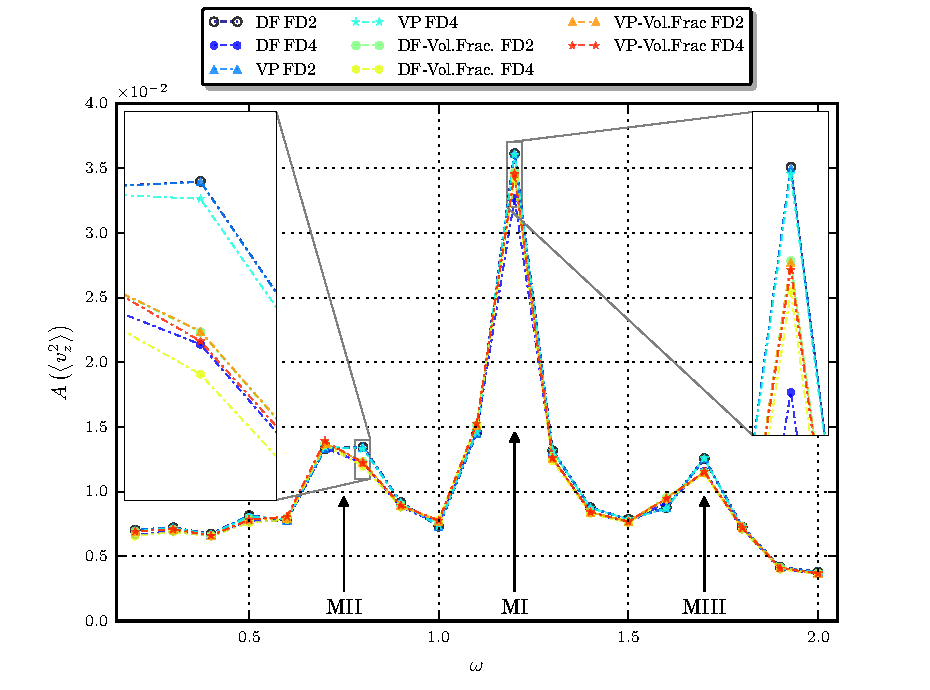
\includegraphics{gfx/cone/cylinder/cylinder.pdf}  \caption{\label{fig:cone:cyl}
    Amplitude of the kinectic energy in $v_z$, as function of the liberating frequency $\omega$.
   For the direct forcing (DF), volume penalization (VP) method with or without Volume Fraction and
      2nd(o2)  and 4th(o4) order finite differences.}
\end{figure}

\bgroup\large
\begin{table}[!b]
\centering
\def\arraystretch{1.5}%
\begin{tabular}{c c c c c}\toprule
            &    m =  1  & m = 2   &    \\ \hline
\midrule
        n=1 &   0.698433         &              0.398913 &    \\
        n=2 & \cellcolor{blue!25}  1.195232         &        \cellcolor{blue!25}      0.754094 &    \\
        n=3 &   1.490715         &              1.042313 &    \\
        n=4 &  \cellcolor{blue!25} 1.660912         &     \cellcolor{blue!25}         1.262759 &    \\
        n=5 &   1.762270         &              1.426587 &    \\
        n=6 &   1.825743         &              1.547435 &    \\ \hline

\bottomrule
\end{tabular}
\caption{Eigenvalues of the (n, m)-inertial modes in a cylinder with aspect ratio $\nicefrac{5}{11}$.
            Possible modes are highlighted.  \label{cone_cyleigenvalues} }
\end{table}
\egroup
\clearpage


\begin{figure}[!t]
  \centering
  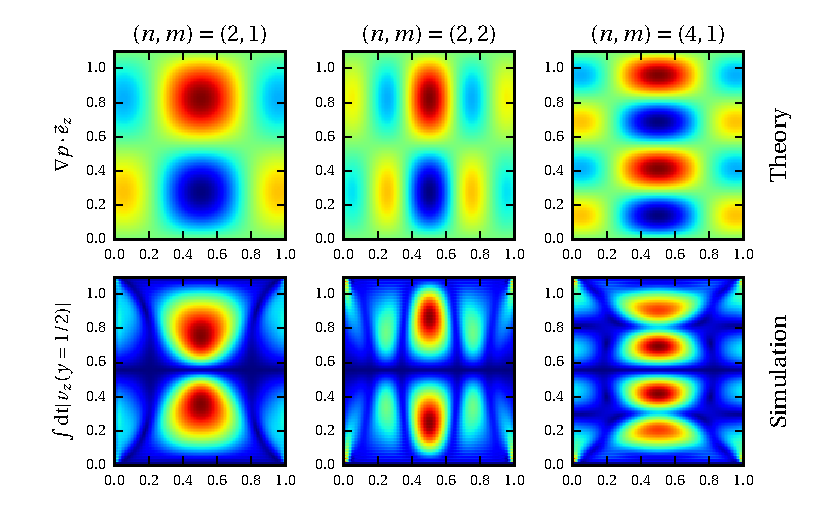
\includegraphics{gfx/cone/cylinder/modes.pdf}  \caption{
      Theoretical inertial modes compared to the absolute velocity component $v_z$.
      For the peaks \RN{1}, \RN{2} and \RN{3}.
      \label{cone:cyl_modes}}
\end{figure}

The theoretical profiles for the inviscid problem, look indeed very similar to the simulated profiles.
The simulation profiles are slightly distorted on the walls of the fluid domain, in
comparison to the theoretical profiles.
For all modes, the number of wave nodes in $z$, and $x$ direction is identical,
 when comparing the theoretical and numerical profiles.

\subsubsection{Helicity}

The computation of the helicity was splited into an integral over the upper and lower half
of the cylinder.  A result for $\omega=1.5$ is exemplarly shown in figure \ref{cone:cyl_helicity}.
In the upper half of the cylinder a negative helicity can be observed, the maximum of the amplitude is of order $10^{-1}$.
In the lower half of the cylinder a positive helicity can be observed, the maximum is of the same order as before.
The helicities are symmetric with respect to zero, thus $H_{\text{up.}} = -H_{\text{low.}}$.
As a result it follows, that the total helicity of the cylinder is zero for all times.

\begin{figure}[!p]
  \centering
  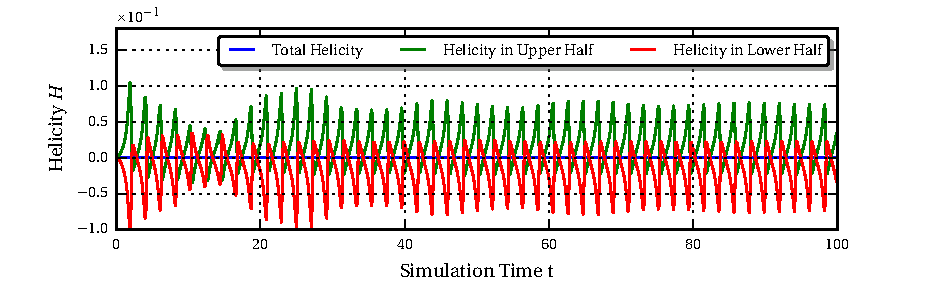
\includegraphics{gfx/cone/cylinder/helicity.pdf}  \caption{
      Time-dependent Helicity $H(t)$ for $\omega=1.5$. The direct forcing method of second order was used.
      \label{cone:cyl_helicity}
      }
  \centering
  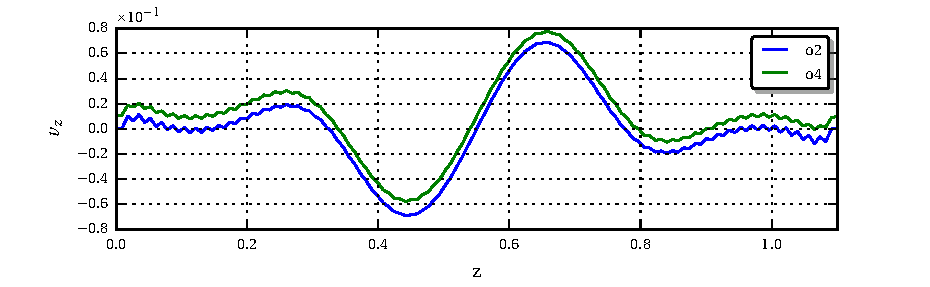
\includegraphics{gfx/cone/cylinder/oscillations.pdf}  \caption{
      Numerical oscillations on the axis $(x,y) = 0.5, 0.5$ and variable $z$.
      For direct forcing method of second (o2) and fourth (o4) order, at $\omega=1.5$.
      \label{cone:cyl_oscillations}
      }
  \centering
  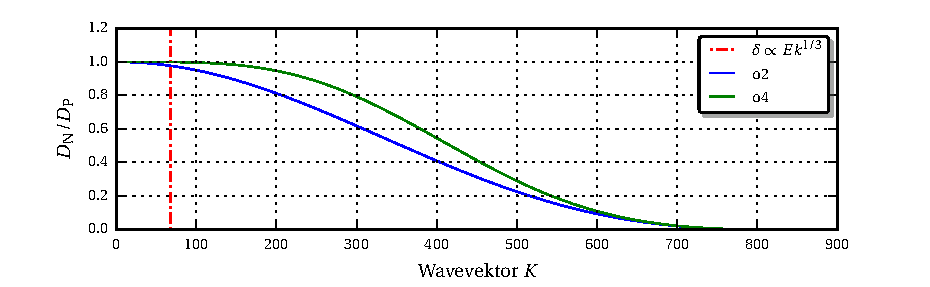
\includegraphics{gfx/cone/cylinder/numvis.pdf}  \caption{
      Ratio $D_N/D_P$ of  numerical viscosity  $D_N$ and physical viscosity computed for $\Ekman=10^{-4}$. For 2nd and 4th- order central differencing schemes.
      The red line indicates the wave vector of an inertial wave node with width $\Ekman^{1/3}$.
      \label{cone:cyl_numvis}
      }
\end{figure}

\subsubsection{Numerical Oscillations}

For all immersed boundary methods numerical oscillations are observable.
Figure \ref{cone:cyl_oscillations} shows this for the 2nd and 4th order direct forcing method and $\omega=1.5$.
The profile is taken along the $z$-Axis at $(x,y)=(\nicefrac{1}{2},\nicefrac{1}{2})$.
It can be noted that the error is larger in the regions near to the wall.
One important detail is that the oscillations are only observable in $z$-direction, not
in th $(x,y)$ plane.
For the 4th order method the upwinding scheme has been used, in contrast to the FTCS-Scheme at 2nd order.
It is visible that the oscillations are slightly diminished, when using the 4th order scheme.

\subsubsection{Numerical Viscosity}

The ratio between the numerical and physical viscosity was computed, according to equation \ref{NUMERIC:NUMVIS}.
The results are shown in figure \ref{cone:cyl_numvis}.
The red bar denotes the wavevektor for the width of an inertial wave, which is $\propto \Ekman^{1/3.}$.
For this value the ratio is $\approx{0.977}$.
For both methods a decrease in the numerical viscosity can  be observed.
At larger wave vektors the 4th order method has a better approximation, than the 2nd order method.
The largest possible wave vektor of the  system is possible for $\lambda = 2\Delta x$,
it follows that $K_{\text{max}} = \nicefrac{2\pi}{\lambda} \approx 402.1$.
\clearpage

\subsection{Discussion}

\subsubsection{Frequency Spectrum}

We assume that the peaks in the frequency spectrum can be identified as inertial modes.
The computed eigenvalues  are close to the peak positions in the spectrum and a first good indicator.
However  the assumption that M\RN{1} could be the (4, 2)-Mode is wrong.
The representation of the averaged $v_z$-component in figure \ref{cone:cyl_modes}, in comparison to the pressure gradient
clarifies that the peak M\RN{1} corresponds to the (2, 1)-Mode.
M\RN{2} corresponds to the (2,2)- Mode and M\RN{3}  to the (4, 1)-Mode.\\
The distortion in the averaged velocity profiles can be explained to the viscous friction from domain boundaries.
The results of the simulations are therefore in a good agreement with the theoretical description of the inviscid case.
\\
An numerical study of the non-linear system was performed by \citep{Sauret2012}.
The inertial modes, which were found in this study confirms our results.
One difference is a slight shift $\approx0.06$ of the eigenvalues,
due to the mistakenly used aspect-ratio .
Furthermore three additional modes were found in this study, which do not occur
in our frequency spectrum.
One explanation for this is that we used a  larger Ekman number in this simulations $\propto10^-4$.
The width of a resonance peak is proportional to the damping rate of the system, in analogy to an harmonic oscillator.
\footnote{Private communication A.Tilgner}
Due to the stronger damping in our simulations the spectrum is smeared out (wie kann man das am besten schreiben?).\\
All methods are able to reproduce these results, with exception of the interpolation method.
Unfortunately we were not able to figure out the reason for the numerical unstability.
The almost indentical errors of the volume penalization and direct forcing method of 2nd order,
indicate that the timestep could be to small.
The velocities local to the domain boundarie are so small, that the damping force (IP-Method) is almost identical
to setting the velocity direct to zero (DF-Method).

\subsubsection{Numerical Oscillations}

The velocities in the system are at least of order $2\cdot10^{-1}$. The resulting Peclet number is
given by
\begin{align}
    \Pe = \frac{0.1\cdot\nicefrac{1}{128}}{\Ekman} =15.625
\end{align}

This value gives a possible explanation for the occurence of oscillations,
since it violates the stability criterion $\Pe<2$.
The improvement from the upwinding scheme, support this assumption.
It still remains unclear why the oscillations only occur in the $z$-direction.
%Furthermore this is in accordanc
%Oscillations usually occur where the velocity gradient is high.
%This can also be seen from the velocity profile of the (2, 2)-mode in figure \ref{cone:cyl_modes}.
%It is possible that the gradient arises from the corners on top and botom of the cylinder
%which is at

\subsubsection{Numerical Viscosity}

The numerical viscosity was computed in order to determine its influence on the system.
For the physical properties of our system, we estimate wavelengths in the range of $1 - \Ekman^{1/3}$.
The error of the numerical viscosity in this range can be neglected.

\subsubsection{Helicity}

The computation shows that the total helicity of the cylinder is zero.
This result is not unexpected.
Due to the axial symmetry in $z$-direction., the helicty in the upper and lower part of the cylinder cancels each other out.

\newpage

\section{Simulation of a Librating Cone}

In this section we will discuss the different numerical simulations, which has been performed
with a librating cone. We begin with the comparison to the experiment performed by \citep{Beardsley1970}.
As a next step we analyse the physical behaviour when performing the transition from a cylinder
to a cone and finally  we will investigate the influence of different offsets on top of the cone.
All simulations performed in this section use the introduced setup with different geometric parameters.
As a IBM we choose the direct forcing  method of second order.

-as a convention we refer to frustom cone etc
-explain method used..
-libration intro immer gleich .. sin etc

\subsection{Simulation of the Experiment}

The setup for this simulation is oriented on the experimental setup given by \citep{Beardsley1970}, which
we disussed in section ().
In the first part of the experiment a plexiglass cylinder of height $H=\SI{19.95}{\centi\meter}$ and a radius of
$r=\SI{19.95}{\centi\meter}$ was used. The apex half angle was set to $24^{\circ}3.7^{\prime}$ degree,
which relates to our setup with $\alpha=65^{\circ}56.3^{\prime}$
For the rotation rate a frequency of $\omega =\SI{6.28}{\radian\per\second}$ was chosen.
As a fluid, water was used, the resulting viscosity,given by \citep{tipler2003}, is $\nu = \SI{1.0}{\milli\pascal\second}$.
The resulting Ekman number is given by

\begin{align}
    \Ekman = \frac{\nu}{\omega r H^2} \approx 7.72\cdot 10^{-6}
\end{align}

In the second part of the experiment the apex of the cone was replaced by a frustum through the
insertion of a bottom plate at the position $z/H = 0.261$.
For the simulation we choose an Ekman number of $\Ekman =  10^{-4}$, since a simulation of higher ekman numbers is
diffcult to realise due to the computational effort.
Furthermore we set $\alpha = \arccos(1/2) = 60^{\circ}$, $H=1$ and $r=0.5$.\\
This means that for $\omega=1$, the propagation of an inertial wave package is parallel to the slope of the cone.
For the offset on top of the cone, we obtain the condition

\begin{align}
    o = H - h_c =  1 - r\tan{\alpha} \approx 0.134
\end{align}

The simulation has two setups in analogy to the experiment.For the second part the bottom plate is set to $h_b=0.25$.
A series of simulations of these systems where performed, with the parameters

\begin{center}
\vspace*{0.7ex}
\begin{tabular}{c|c|c|c|c|c|c }
%\begin{tabular}{p{0.1\linewidth}| p{0.1\linewidth}| p{0.1\linewidth}|  p{0.1\linewidth}| p{0.1\linewidth}| p{0.1\linewidth} }
$ \leftarrow  \omega \rightarrow $ & $\Delta t$ & $\Delta x$ & $c^2$ & \Ekman  & $l_x, l_y, l_z$ & $T_{end}$\\
\hline
$[0.2,\; 2], \Delta w = \nicefrac{1}{10}$ & $10^{-5}$ & $\nicefrac{1}{128}$ & 500 & $10^{-4}$  & (\{1, 0.75\}, 1, 1) & 100\\
\end{tabular}
\vspace*{0.7ex}
\end{center}

\clearpage
%\begin{figure}[!tp]
%  \begin{minipage}[c]{0.6\textwidth}
%      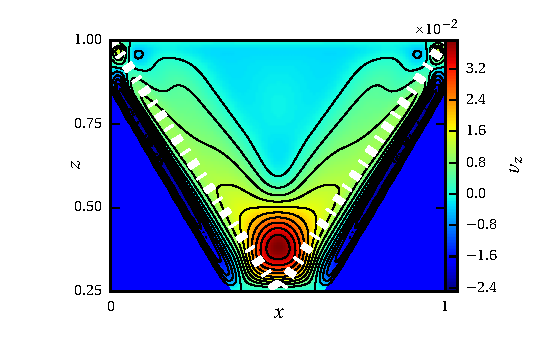
\includegraphics{gfx/cone/experiment/contour.pdf}\label{fig:mask_vp}
%  \end{minipage}\hfill
%  \begin{minipage}[c]{0.3\textwidth}
%  \caption{Stability regions for $\Omega_s$ for different Runge-Kutta methodsi
%    Stability regions for $\Omega_s$ for different Runge-Kutta methodsi
%  }
%  \label{fig:num_rkstab}
%  \end{minipage}
%\end{figure}
%
%\begin{figure}[!tp]
%  \begin{minipage}[c]{0.3\textwidth}
%  \caption{Stability regions for $\Omega_s$ for different Runge-Kutta methods
%  Stability regions for $\Omega_s$ for different Runge-Kutta methodsi
%  }
%  \label{fig:num_rkstab}
%  \end{minipage}
%  \hfill
%  \begin{minipage}[c]{0.6\textwidth}
%      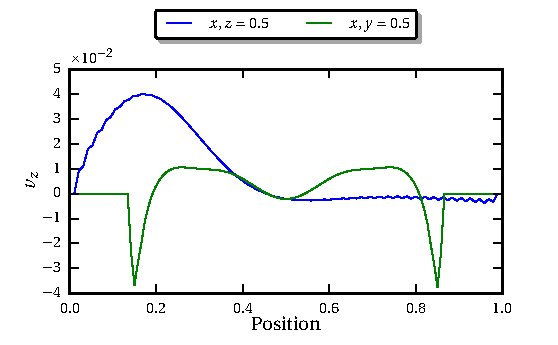
\includegraphics{gfx/cone/experiment/error.pdf}\label{fig:mask_vp}
%  \end{minipage}
%\end{figure}

\begin{figure}[!bp]
  \centering
  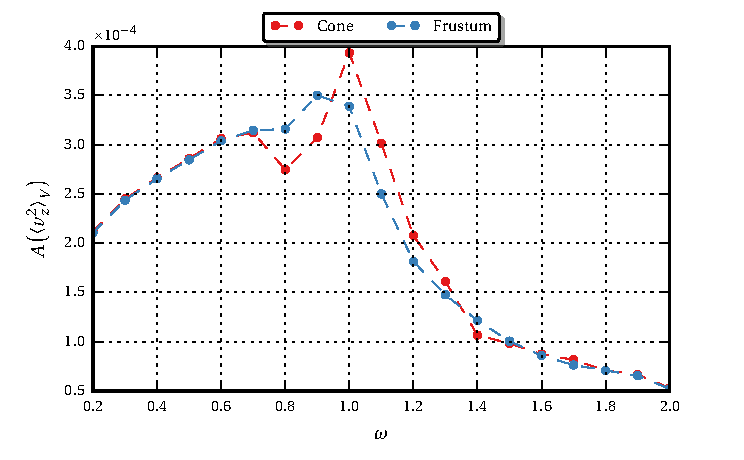
\includegraphics{gfx/cone/experiment/experiment.pdf}
  \caption{Amplitude $A\left(\left<v^2_z\right>_V\right)$ as a function of the libration frequency $\omega$,
            for a cone and a frustum.  \label{fig:cone_expseries} }
\end{figure}

\subsubsection{Results \& Discussion}
\label{cone:exp}

The results of the simulations are shown in figure \ref{fig:cone_expseries}.
For both cases, the frustum and the cone, we can observe an increase in $A\left(\left<v^2_z\right>_V\right)$
from $\approx 2\cdot10^{-4}$ at $\omega=0$ to  $\approx 3.4\cdot10^{-4}$ for the frustum and $\approx 4\cdot10^{-4}$ for the cone,  at $\omega=1$.
From here one the Amplitude decreases to $\approx 5\cdot10^{-5}$ at $\omega=2$.\\
A difference between the two setups can be observed in the surrounding area of $\omega=1$.
For the cone the increase of the amplitude is interrupted at $\omega=0.6$, a minimum can be observed at $\omega=0.8$, followed by
a peak at $\omega=1$. For the frustum the minium is not directly visible but it can be noted that the
amplitude does not increase as much at $\omega=0.7$, as for lower frequencies.\\
The maximum occurs at $\omega=0.9$, in comparison to the cone we see an increase in the amplitude of $\approx 5\cdot10^{-5}$.
However, it has to be considered, that due do the stepwidth of $\Delta \omega = 0.1$, the exact position of the maxima is
not apparent.\\
One possible assumption, regarding the position of the maximum with respect to the frequency, is that
the expansion of the frustum with a tip  results in a shift to lower frequencies.
The left shift in the decrease for $\omega > 1$ furthermore supports this idea.\\
Overall it appears that the (spectrum) can be divided into two domains $\Omega_1~=~\{0\leq\omega<1$\} and $\Omega_2~=~\{1\leq\omega\leq2\}$.
This result is not unexpected, since we choose the slope $\alpha$ of the cone such that for $\omega=1$, it is parallel
do the group velocity $\vec{c}_{g}$.
For $\omega\in\Omega_1$ the results for both setups are similar, since in this domain, the cone tip does not act as an attractor.
An inertial wave propagates the top, after a reflection on the side of the cone.
Hence, for both setups we obtain a similar (spectrum).
The differences occur when $\omega$ is reaching the critical slope, in this scenario an inertial wave propating from the
top edges, travereses directly into the apex of the cone, or is reflected slightly at he bottom plate of the frustum.
As a results we see the increase in the amplitude.
For $\omega\in \Omega_2$ we would expect further reflections for the frustum, however the similar
decay of the amplitude refutes this assumption.\\
The results of the simulation do not match with the ones of the experiment we discussed in section ().
A possible explanation we want to propose here, is the use of a different Ekman number, which is of order $10^{-4}$ in contrast
to the one of the experiment of $10^{-5}$.
As a consequence the width of an inertial wave packet, given by $\propto \Ekman^{1/3} \approx 2\cdot10^{-2}$ (see \citep{} or section...),
is around twice the size as in the experiment. We assume that as a results a wave reflecting on the bottom of the frustum
is strongly damped due to wall friction.
DISCUSS T:\\
damping  could be propt $\Ekman \vec{K}$.

\subsection{Transition to from a Cylinder to a Cone}

We now want to further investigate the results from the previous simulation.
The assumption was made, that the inserted bottom plate is to narrow to support an efficient reflection
of inertial waves, due to frictional losses at the bottom of the cone. Thus, the next objective would be to
test the influence of different gap radii $r$.\\
We propose a setting where we begin with the possible largest bottom gap, which is $r=0.5$.
As a next step we iteratively decrease the size of the gap by $\Delta r = 0.125$ until $r=0$ is reached.
An alternative approach to this woudld be to change the offset from the bottom of the cone, which would result in a constant
slope but different heights of the simulation domain.
The influence on the simulation domain is shown in figure ()(b).
For $r=0.5$ the domain is given by a cylinder, which than transforms into a cone with a frustum and finally with an apex for $r=0$.
The main simulation parameters are given by

\begin{center}
\vspace*{0.7ex}
\begin{tabular}{c|c|c|c|c|c|c|c }
%\begin{tabular}{p{0.1\linewidth}| p{0.1\linewidth}| p{0.1\linewidth}|  p{0.1\linewidth}| p{0.1\linewidth}| p{0.1\linewidth} }
$\leftarrow r \rightarrow$ & $ \leftarrow  \omega \rightarrow $ & $\Delta t$ & $\Delta x$ & $c^2$ & \Ekman  & $l_x, l_y, l_z$ & $T_{end}$\\
\hline
$[0,\; 0.5], \Delta r =0.125$ & $[0.2,\; 2], \Delta w = \nicefrac{1}{10}$ & $10^{-5}$ & $\nicefrac{1}{128}$ & 500 & $10^{-4}$  & (1, 1, 1) & 100\\
\end{tabular}
\vspace*{0.7ex}
\end{center}
%
%\subsubsection{Results \& Discussion}
%\begin{figure}[!bp]
%      \begin{minipage}[c]{0.4\textwidth}
%      \centering
%        \resizebox{0.8\textwidth}{!}{
%       \import{gfx/cone/transition//}{attractor.pdf_tex}
%      }
%      \end{minipage}\hfill
%  \begin{minipage}[c]{0.6\textwidth}
%      \caption{
%          Wave attractor in a cylinder $\left(\text{\colorbox{green}{\textcolor{green}{o}}{\null}}\right)$
%          and shifted\\ attractor $\left(\text{\colorbox{red}{\textcolor{red}{o}}{\null}}\right)$
%          for $r<0.5$. To maintain the same attractor the point of reflection has to be at the same height $h_r$.
%      }
%      \label{cone:theorie}
%      \end{minipage}\hfill
%\end{figure}



\subsubsection{Results \& Discussion}

The results of the simulations are shown in figure \ref{fig:cone:transition}.
For $r=0$ we can see the inertial modes of a librating cylinder, which is in accordance
to the results we discussed in section \ref{cone:sec:lib_cylinder}.
With an decrease of the radius we can observe a change in the position and amplitude of the
inertial modes. We want to exemplarly discuss this pattern for the (2, 2) mode at $\omega=1.3$, where it is the best visible.
For all other modes the transition results in a similar behvavior.\\

\begin{figure}[!pt]
  \centering
  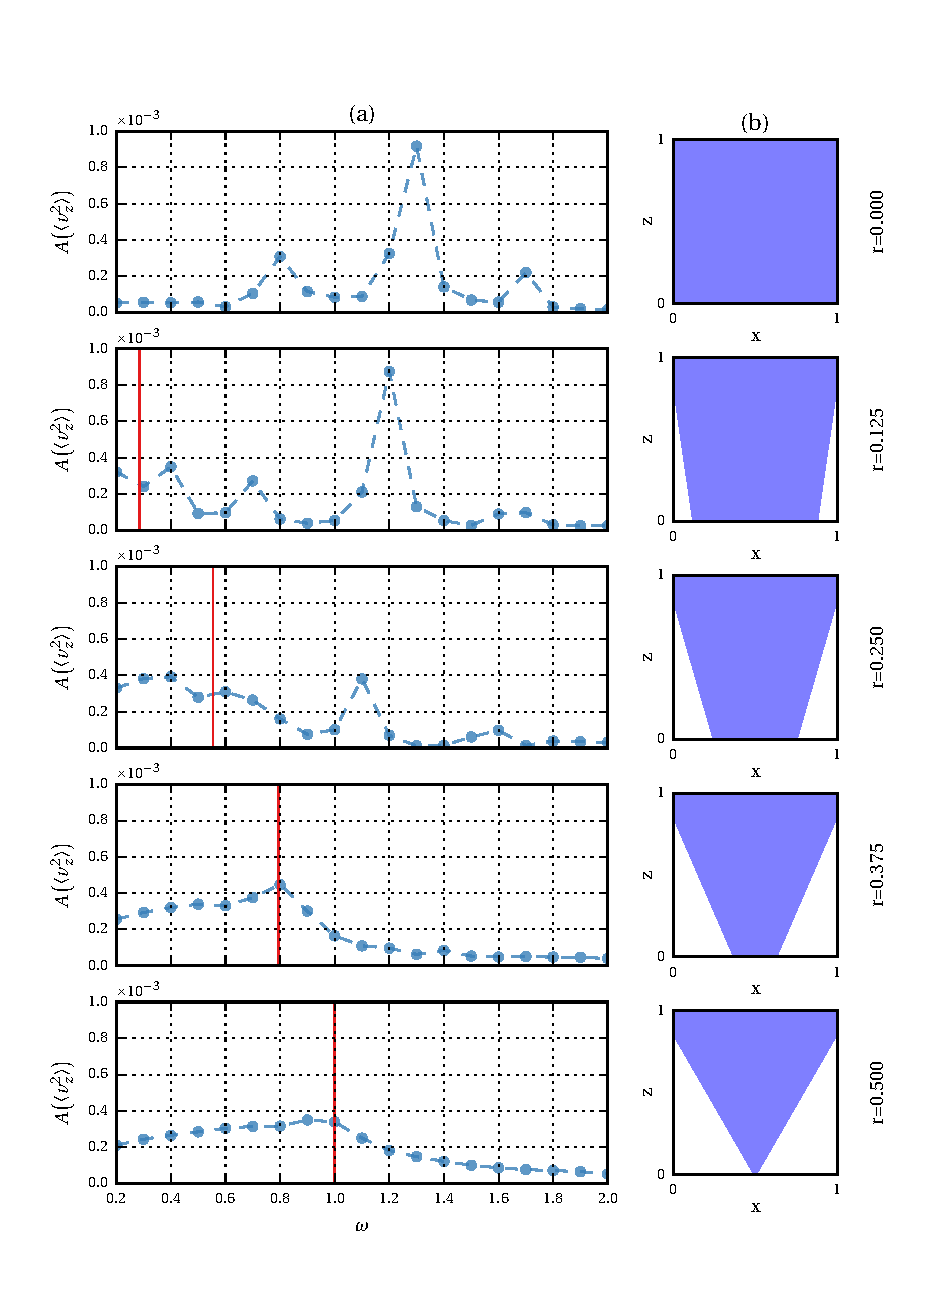
\includegraphics{gfx/cone/transition/transition.pdf}
  \caption{\label{fig:cone:transition}
    Simulation of
  }
\end{figure}

The decrease of the radius leads to a shift to lower frequencies of the (2, 2) mode,
from $r=0$ to $r=0.375$ it is of the order $\Delta \omega=0.1$.
Furthermore we can see, that during the transition a damping of the mode occurs.
For $r=0.5$ the amplitude is of order $\approx8.9\cdot10^{-3}$, for $r=0.375$ it is
$\approx8.9\cdot10^{-3}$ and for $r=0.25$ we obtain $\approx3.8\cdot10^{-3}$.\\
Whereas the first decrease of the radius does not significantly affect the amplitude,
the second decrease leads to a strong damping to less than half of the original size.
With a further decrease in $r$, the (2, 2) mode is annihilated.
\footnote{ for the possible (1, 2) mode we still can observe a slight increase of the amplitude at $r=1.4$}
One possible explanation for the shift can be given
by having a look at the inertial mode structure, for different radii as shown in figure \ref{fig:cone:phase}.\\
For $r=0.5$ we have an inertial mode, which is symmetric to the plane $h/2$.
In this plane, the waves excited from the bottom and top of the cylinder, annihilate each other and form a wave node.
An decrease of radius breaks the axial symetrie of the inertial mode.
As a result only a distorted version of the mode can exist, where the center of the wave node
is given by the intersection of the diagonals from the top to the bottom edges of the frustum.
In order to obtain the new shape it is necessary to increase the propagation angle $\Theta$,
which is equivalent to lowering the libration frequency.
We can furthermore say that for $r \rightarrow 0$, the center given by

\begin{align}
c  = r \frac{h}{r+\nicefrac{l_x}{2}}
\end{align}

converges against zero, hence a mode cannot exist in this state.
Beside the changes of the inertial modes it can be noted, that simultaneously to the decrease of the radius,
a lift of the amplitudes at lower frequencies occurs.
The vertical lines in figure \ref{fig:cone:transition} are set to the position $\omega=\Theta$.
The area $\omega<\Theta$ can again be associated with the frequency domain, where the wave propagation angle $\Theta$ is larger than
the  slope of the cone $\alpha$ and waves propgate to the top, up on reflection on the slope.
For $r=0$ we have the indentical setup to the simulation in section \ref{cone:exp}.

\begin{figure}[!pt]
  \centering
  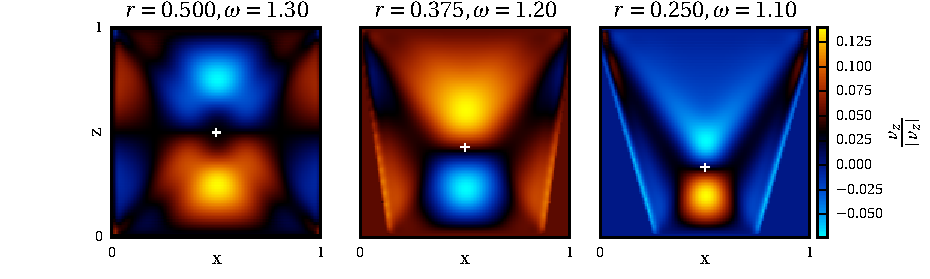
\includegraphics{gfx/cone/transition/phase.pdf}
  \caption{\label{fig:cone:phase}
    Simulation of
  }
\end{figure}

\clearpage

\subsection{Librating Cone with Differing Offsets at the Top}
\subsubsection{Introduction}

A a closure, this section represents the results computed with a new modified setup, which are more in accordance
with the experiment we introduced.
The improvements are based on the results and insights, which were gained from the previous simulations of the librating cone.
We want to adress the  most important points

\begin{itemize}
    \item The radius of the bottom plate of the frustum has a strong influence on
          the reflection of inertial waves.
          Due to the Ekman number of $\Ekman=10^{-4}$ we use, which is one order of magnitude
          above the experiment we assumed that a stronger damping acts on an inertial wave
          at the bottom plate.

    \item As a second point, we want to adress the influence of the offset on top of the cone,
          which has been left out from any discussion so far.
          It can be assumed this offset has a strong influence
          on inertial wave propagation.
          In particular for the intervall $\Theta<\alpha$, where wave super-critical reflection into the top corners occurs.
          In the case where $O=0$, the corners of the cone act as an attractor, as pointed out in figure \ref{cone:img_finalattractor}.
          For small gap sizes it applies that a inertial wave will be damped, in analogy to the bottom gap.
\end{itemize}

As a conlusion a larger gap radius $r$ for the bottom plate, will be introduced.
The exact influence of the offset is unknow, therefore we propose a series of simulations with different offsets.

\begin{figure}[!bp]
      \centering
        \resizebox{0.9\textwidth}{!}{
       \import{gfx/cone//}{comparison.pdf_tex}
      }
      \caption{
          Wave reflection for $o>0$ in the upper edges of the cone (left) and
          an attractor for $o=0$ (right), in the upper edges of the cone.
      \label{cone:img_finalattractor}
      }
\end{figure}

\subsubsection{Setup}

In this setup the radius $r$ is implitciy set by changing the height of the
bottom plate to $h_b=0.375$.  The resulting radius is $r \approx 0.22$.
This is done in order to maintain the constant slope of $\alpha=60$,
which is parallel to an inertial wave for $\omega=1$.
An additional offset is added to the default one,
varying in the range of $h_+ = [0, 0.5]$ with a stepsize of $\Delta h_+ = \nicefrac{1}{5}$.
The complete offset at the top is $O =  (\nicefrac{1}{2})\tan{\nicefrac{\pi}{3}}{2}+ h_+$.
The main simulation parameters are given by

\begin{center}
\vspace*{0.7ex}
\begin{tabular}{c|c|c|c|c|c|c|c }
%\begin{tabular}{p{0.1\linewidth}| p{0.1\linewidth}| p{0.1\linewidth}|  p{0.1\linewidth}| p{0.1\linewidth}| p{0.1\linewidth} }
$\leftarrow h_+\rightarrow$ & $ \leftarrow  \omega \rightarrow $ & $\Delta t$ & $\Delta x$ & $c^2$ & \Ekman  & $l_x, l_y, l_z$ & $T^*_{end}$\\
\hline
$[0,\; 0.5], \Delta h_+ =0.125$ & $[0.2,\; 2], \Delta w = \nicefrac{1}{20}$ & $10^{-5}$ & $\nicefrac{1}{128}$ & 500 & $10^{-4}$  & (1, 1, $1+h_+$) & $\gtrsim100$\\
\end{tabular}
\vspace*{0.7ex}
\end{center}

It should be noted that a higher resolution for the frequency was used compared to the previous simulations.
The total simulation time $T^*_{end.}$ is marked as $\gtrsim 100$, here we want to introduce the modification

\begin{align}
    T_{\text{end.}}^* = \underbrace{\Bigl\lfloor\left(\text{T}_{\text{end}}\frac{\omega}{2\pi}\right)\Bigr\rfloor}_{
        \text{Floor}
        }\frac{2\pi}{\omega} + \frac{2\pi}{\omega}
\end{align}

As a consequence the endtime  of all frequencies, is set to the point where the librating force is crossing zero.
The scenario we want to study from there on is the decay of inertial waves.
To achieve this we continue a simlations with the previously computed endstates and set the libration amplitude $\epsilon$ to zero.
With the use of the modified endtime, we assume all that all intertial waves are
approximately in the same phase with respect to their libration frequency.
The simulation parameters changes according to

\begin{center}
\vspace*{0.7ex}
\begin{tabular}{c|c|c|c}
%\begin{tabular}{p{0.1\linewidth}| p{0.1\linewidth}| p{0.1\linewidth}|  p{0.1\linewidth}| p{0.1\linewidth}| p{0.1\linewidth} }
$\leftarrow h_+ \rightarrow$ & $ \leftarrow  \omega \rightarrow $ & $\epsilon$ & $T_{\text{end}}$\\
\hline
 see \ref{p.xx} & see \ref{p.xx} & 0 & 150\\
\end{tabular}
\vspace*{0.7ex}
\end{center}

For h and w choose specific points as explained in the discussion ( ?)
As a last step we will repeat a part of the simulations for an Ekman number of $\Ekman = 10^{-3}$
-hd simulaiton nachträglich

\clearpage

\subsection{Results}
\subsubsection{Spectrum for the Simulation with Different Offsets}

The results for this simulation are shown in figure \ref{fig:cone:finaltransition}.
On the left side of the plot  the frequency spectrum is shown, the right side illustrates the used geometry.
The height $h_+$ is in descending order, from top to bottom.
Each plot contains two spectra, one for the cone  and the other one for the frustum.
We beginn with a qualitative description of the curves for the frustum.\\
At all heights $h_+$, several resonance modes can be observed. For now we will consider the case where ${h_+=0.25}$.
For this height the largest peaks occur in the spectrum, which are numerated here in decreasing order of the amplitude.\\
The largest mode (\RN{1}) can be observed at a frequency $\omega=1.05$, the amplitude is of the order $5\cdot10^{-4}$.
The second mode (\RN{2}) can be found at $\omega=0.9$ of order $3.7\cdot10^{-4}$, followed by
a possible mode (\RN{3}) at $\omega=0.5$ of order $2.8\cdot10^{-4}$.
On the right side of the spectrum there are two possible small resonances at $\omega=1.7$ and $\omega=1.5$ (\RN{4}, \RN{5}).
For the case $h_+=0.5$  we can see small additional resonances  (\RN{6}) at $\omega=1.8$ and (\RN{7}) at $\omega=0.55$,
the latter is embedded in the slope of the (\RN{3}) mode.
For all peaks (except (\RN{7}), it can be noted, that a lowering of the offset height $h_+$ results
into a shift towards higher frequencies. This can be best seen when looking at the peaks (\RN{1}) and (\RN{2}).\\
Let us now consider the results of the cone.
Above the critical slope $\alpha=\theta$ nearly all resonances are eliminated. One exception is the (\RN{4}) mode for
$h_+=0.5$ and $h_+=0.375$. Another exepction is at the position of the previous (\RN{1}) mode of the frustum.
For $h_+=0.5$ (see \textbf{O}) a small increase in the amplitude can be observed.
On the left side of the critcal slope we can identfiy the (\RN{3})-peak
at the same frequency and same order as for the frustum. To the left side of this point the spectrum for
the cone and the frustum are similar.

\begin{figure}[!bp]
  \centering
  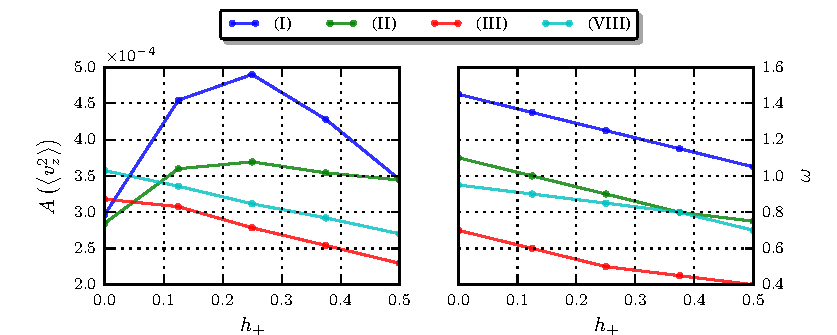
\includegraphics{gfx/cone/final/amp_pos.pdf}
  \caption{
      \label{fig:cone:finalampmax}
    top.
    }
\end{figure}

\begin{figure}[!pt]
  \centering
  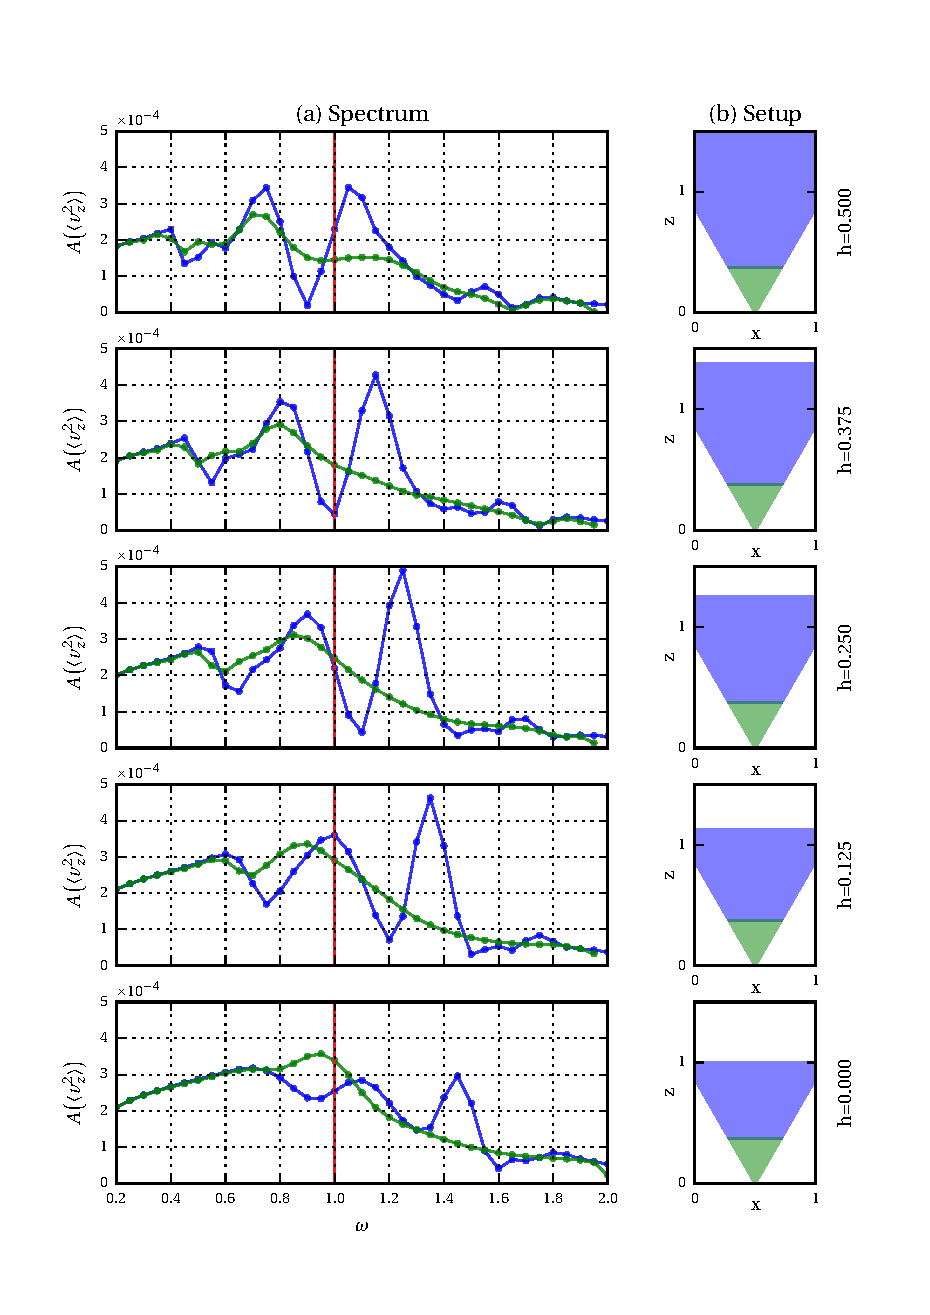
\includegraphics{gfx/cone/final/transition.pdf}
  \caption{
      \label{fig:cone:finaltransition}
    Simulation of a cone (green) and a frustum (blue) for different offsets at the
    top.
    }
\end{figure}
\clearpage

Furthermore at the position of peak (\RN{2}) of the cone, we now see a slightly diminshed mode \RN{8}.
The maximum is at the same frequency at $h_+=0.5$ but diverges slightly with an decrease of the height $h_+$.\\
comparison:
-symetrie h0.5 mode 1 2
-asymertie mode 1 h0.5

-comper cone to frustum
-offset propt to peak shift to left
-amplitude
-plot peak shift

-plot amplitude shift
-discuss plot

qualitative:
-bestimmung maxima und amplituden
-dargestellt in plot ...
- discussion
-anstieg m1 und m2
-abfall m3 und m8
relativ linear abfall für alle moden
-allerdings auflösung dafür nicht gut
-comper cone to frustum
-offset propt to peak shift to left
-amplitude

-plot peak shift
-plot amplitude shift

-discuss plot



\subsubsection{Helicity}

-helicity results shown in figuren..
- global or acc
- nicht so ins detail gehen
- important features
- steigung beim critical slope
- diskutiere bereiche links rechts
- sehr kleine helizität

\subsubsection{Decay rates}

-ablkingraten für maxima ploten und vergleichen den verlauf
-resultate fit schnell gemacht
- positionen erläutern
- ablkingraten dargestellt in figure so und so
- diskussion

\subsubsection{High Resolution Comparison}

\subsubsection{Larger Ekman number}

-test alte ergebnisse evtl erläutern

\clearpage

\subsection{Discussion}

\subsubsection{Spectrum for the Simulation with Different Offsets}

-links von m3 gleiches spectrum bild strahlengang bei m3
-shift geometrie erklärung
-vergleich zylinder mode evlt im paper nachschauen
-gucke animationen alle moden im vergeich beispielbilder  cone/frustom vgl

-fehler 8er mode bild zylinder theorie reibung

\subsubsection{Helicity}

-helicity is sehr klein system ist nicht gut geignet für einen dynamo?
-check fehler berechnung l2 norm

\subsubsection{Decay rates}



-results erstmal machen
-wichtig diskussion turbulenz!

\subsubsection{Larger Ekman number}

\subsubsection{Ray Tracer}


\section{Summary}
\subsection{Summary}
freeslip besser

In addition to default helicity compuattion, we will also compute

Furthermore we will compute the normalized helicity of the system given by
in the accelerated frame of reference and also for the inertial system with an additional offset in the velocity
given by $\vec{u} = \vec{u}|_{\text{rot.}} + \Omega(t) \times \vec{r}$.

All methods were able to reproduce the modes M\RN{1}, M\RN{2} and M\RN{3},
The only exeption is the interpolation method, which is numerical unstable.
This is a little bit of a disappointing results, since this methods tends to contain
the smallest numerical error.
Another point which should be consider for future simulations are the numerical oscillations.
This could be fixed with an improvement method, for example with the use of free slip boundaries
-kleinerer grient an den seiten
-abeir schwieriger zu implementiern
As an alternative a higher resolution  could be used, which is computational expensive.

what have we done
zusammen fassung results
- good first step
-erflogreich in übereintstimmung mit der simulation
-für kleine eckman zahlen simulairen interessant um mehr moden zu finden
outlook hd simulationen
